% Created by tikzDevice version 0.10.1 on 2016-02-27 13:08:36
% !TEX encoding = UTF-8 Unicode
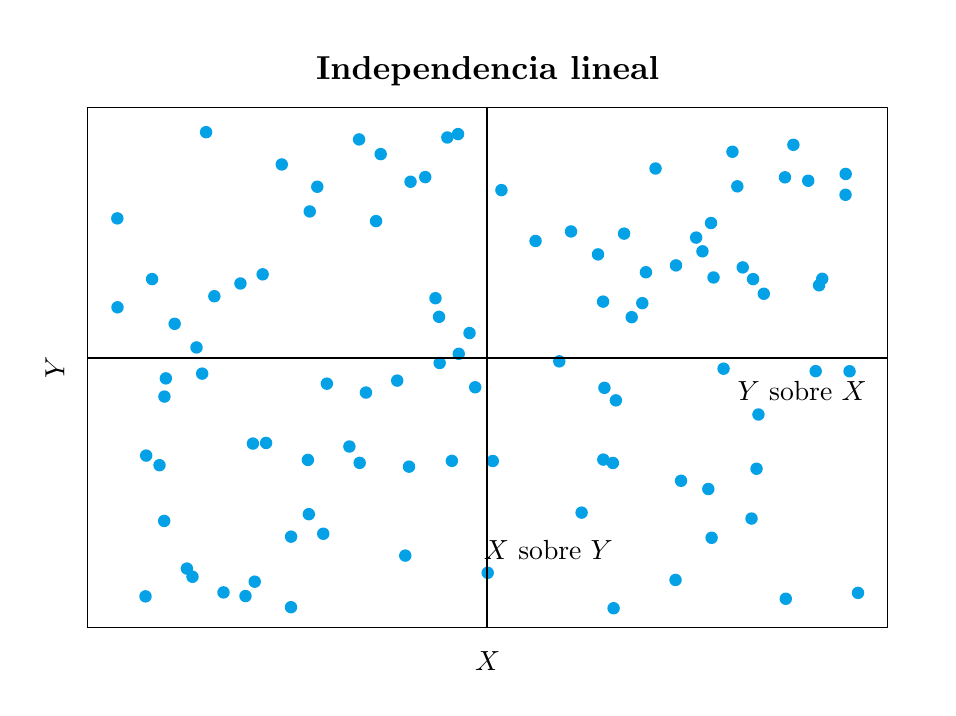
\begin{tikzpicture}[x=1pt,y=1pt]
\definecolor{fillColor}{RGB}{255,255,255}
\path[use as bounding box,fill=fillColor,fill opacity=0.00] (0,0) rectangle (325.21,238.49);
\begin{scope}
\path[clip] ( 21.68, 21.68) rectangle (310.76,209.58);
\definecolor{fillColor}{RGB}{5,161,230}

\path[fill=fillColor] (245.95, 71.78) circle (  2.25);

\path[fill=fillColor] (147.36,140.74) circle (  2.25);

\path[fill=fillColor] (116.25, 87.14) circle (  2.25);

\path[fill=fillColor] (148.86,117.32) circle (  2.25);

\path[fill=fillColor] (125.89,168.59) circle (  2.25);

\path[fill=fillColor] ( 84.91,149.36) circle (  2.25);

\path[fill=fillColor] ( 42.58, 33.00) circle (  2.25);

\path[fill=fillColor] (101.26, 82.30) circle (  2.25);

\path[fill=fillColor] (122.24,106.64) circle (  2.25);

\path[fill=fillColor] (284.75,114.37) circle (  2.25);

\path[fill=fillColor] (218.26,133.88) circle (  2.25);

\path[fill=fillColor] (192.10,117.91) circle (  2.25);

\path[fill=fillColor] (236.09, 74.76) circle (  2.25);

\path[fill=fillColor] (127.56,192.80) circle (  2.25);

\path[fill=fillColor] (212.54,103.82) circle (  2.25);

\path[fill=fillColor] (282.06,183.18) circle (  2.25);

\path[fill=fillColor] (247.83,148.22) circle (  2.25);

\path[fill=fillColor] ( 67.46,141.44) circle (  2.25);

\path[fill=fillColor] (226.88,187.60) circle (  2.25);

\path[fill=fillColor] (206.09,156.56) circle (  2.25);

\path[fill=fillColor] (155.76,120.64) circle (  2.25);

\path[fill=fillColor] (211.47, 81.20) circle (  2.25);

\path[fill=fillColor] ( 53.11,131.48) circle (  2.25);

\path[fill=fillColor] (196.34,164.85) circle (  2.25);

\path[fill=fillColor] ( 61.01,122.93) circle (  2.25);

\path[fill=fillColor] (263.37, 79.11) circle (  2.25);

\path[fill=fillColor] (200.17, 63.25) circle (  2.25);

\path[fill=fillColor] (101.60, 62.69) circle (  2.25);

\path[fill=fillColor] ( 49.33, 60.25) circle (  2.25);

\path[fill=fillColor] (258.38,151.86) circle (  2.25);

\path[fill=fillColor] (171.19,179.79) circle (  2.25);

\path[fill=fillColor] (247.14, 54.17) circle (  2.25);

\path[fill=fillColor] ( 95.18, 54.57) circle (  2.25);

\path[fill=fillColor] ( 57.55, 43.03) circle (  2.25);

\path[fill=fillColor] (273.65,184.41) circle (  2.25);

\path[fill=fillColor] (104.65,181.01) circle (  2.25);

\path[fill=fillColor] (287.12,147.74) circle (  2.25);

\path[fill=fillColor] (243.83,157.68) circle (  2.25);

\path[fill=fillColor] (119.75,198.11) circle (  2.25);

\path[fill=fillColor] (266.00,142.34) circle (  2.25);

\path[fill=fillColor] (261.56, 61.11) circle (  2.25);

\path[fill=fillColor] ( 86.15, 88.43) circle (  2.25);

\path[fill=fillColor] ( 70.76, 34.42) circle (  2.25);

\path[fill=fillColor] (136.45, 47.72) circle (  2.25);

\path[fill=fillColor] (133.53,110.96) circle (  2.25);

\path[fill=fillColor] (101.93,172.08) circle (  2.25);

\path[fill=fillColor] ( 76.88,146.05) circle (  2.25);

\path[fill=fillColor] ( 59.55, 40.08) circle (  2.25);

\path[fill=fillColor] ( 64.47,200.72) circle (  2.25);

\path[fill=fillColor] ( 42.82, 83.87) circle (  2.25);

\path[fill=fillColor] (106.81, 55.62) circle (  2.25);

\path[fill=fillColor] (296.99,114.33) circle (  2.25);

\path[fill=fillColor] (161.71,108.55) circle (  2.25);

\path[fill=fillColor] (295.53,178.10) circle (  2.25);

\path[fill=fillColor] (137.80, 79.86) circle (  2.25);

\path[fill=fillColor] ( 95.15, 29.08) circle (  2.25);

\path[fill=fillColor] (166.23, 41.51) circle (  2.25);

\path[fill=fillColor] (300.05, 34.25) circle (  2.25);

\path[fill=fillColor] (295.59,185.63) circle (  2.25);

\path[fill=fillColor] (254.67,193.65) circle (  2.25);

\path[fill=fillColor] ( 81.39, 88.20) circle (  2.25);

\path[fill=fillColor] (276.68,196.16) circle (  2.25);

\path[fill=fillColor] (234.27,152.59) circle (  2.25);

\path[fill=fillColor] (215.51,164.07) circle (  2.25);

\path[fill=fillColor] ( 47.64, 80.39) circle (  2.25);

\path[fill=fillColor] (251.46,115.26) circle (  2.25);

\path[fill=fillColor] (119.96, 81.23) circle (  2.25);

\path[fill=fillColor] (159.66,128.14) circle (  2.25);

\path[fill=fillColor] ( 49.94,111.76) circle (  2.25);

\path[fill=fillColor] (234.10, 38.92) circle (  2.25);

\path[fill=fillColor] (223.41,150.11) circle (  2.25);

\path[fill=fillColor] (183.52,161.41) circle (  2.25);

\path[fill=fillColor] (108.11,109.85) circle (  2.25);

\path[fill=fillColor] ( 44.96,147.64) circle (  2.25);

\path[fill=fillColor] (273.95, 32.13) circle (  2.25);

\path[fill=fillColor] (262.12,147.63) circle (  2.25);

\path[fill=fillColor] (148.65,134.00) circle (  2.25);

\path[fill=fillColor] (208.01, 82.41) circle (  2.25);

\path[fill=fillColor] (208.41,108.35) circle (  2.25);

\path[fill=fillColor] (246.92,167.90) circle (  2.25);

\path[fill=fillColor] (241.55,162.63) circle (  2.25);

\path[fill=fillColor] (151.64,198.81) circle (  2.25);

\path[fill=fillColor] ( 78.71, 33.10) circle (  2.25);

\path[fill=fillColor] (211.73, 28.70) circle (  2.25);

\path[fill=fillColor] ( 63.05,113.48) circle (  2.25);

\path[fill=fillColor] ( 82.04, 38.30) circle (  2.25);

\path[fill=fillColor] (168.07, 81.91) circle (  2.25);

\path[fill=fillColor] ( 32.46,137.44) circle (  2.25);

\path[fill=fillColor] ( 49.41,105.19) circle (  2.25);

\path[fill=fillColor] (143.66,184.50) circle (  2.25);

\path[fill=fillColor] (155.51,200.04) circle (  2.25);

\path[fill=fillColor] (153.29, 81.95) circle (  2.25);

\path[fill=fillColor] (138.35,182.81) circle (  2.25);

\path[fill=fillColor] (207.92,139.50) circle (  2.25);

\path[fill=fillColor] (264.07, 98.71) circle (  2.25);

\path[fill=fillColor] (256.43,181.16) circle (  2.25);

\path[fill=fillColor] ( 32.39,169.58) circle (  2.25);

\path[fill=fillColor] ( 91.82,189.06) circle (  2.25);

\path[fill=fillColor] (222.09,138.94) circle (  2.25);

\path[fill=fillColor] (285.97,145.40) circle (  2.25);
\end{scope}
\begin{scope}
\path[clip] (  0.00,  0.00) rectangle (325.21,238.49);
\definecolor{drawColor}{RGB}{0,0,0}

\node[text=drawColor,anchor=base,inner sep=0pt, outer sep=0pt, scale=  1.20] at (166.22,219.84) {\bfseries Independencia lineal};

\node[text=drawColor,anchor=base,inner sep=0pt, outer sep=0pt, scale=  1.00] at (166.22,  6.08) {$X$};

\node[text=drawColor,rotate= 90.00,anchor=base,inner sep=0pt, outer sep=0pt, scale=  1.00] at ( 13.28,115.63) {$Y$};
\end{scope}
\begin{scope}
\path[clip] (  0.00,  0.00) rectangle (325.21,238.49);
\definecolor{drawColor}{RGB}{0,0,0}

\path[draw=drawColor,line width= 0.4pt,line join=round,line cap=round] ( 21.68, 21.68) --
	(310.76, 21.68) --
	(310.76,209.58) --
	( 21.68,209.58) --
	( 21.68, 21.68);
\end{scope}
\begin{scope}
\path[clip] ( 21.68, 21.68) rectangle (310.76,209.58);
\definecolor{drawColor}{RGB}{0,0,0}

\path[draw=drawColor,line width= 0.8pt,line join=round,line cap=round] ( 21.68,119.08) -- (310.76,119.08);

\path[draw=drawColor,line width= 0.8pt,line join=round,line cap=round] (166.07, 21.68) -- (166.07,209.58);

\node[text=drawColor,anchor=base,inner sep=0pt, outer sep=0pt, scale=  1.00] at (188.18, 46.25) {$X$ sobre $Y$};

\node[text=drawColor,anchor=base,inner sep=0pt, outer sep=0pt, scale=  1.00] at (279.87,103.64) {$Y$ sobre $X$};
\end{scope}
\end{tikzpicture}
